%----------------------------------------------------------------------------------------
%----------------------------------------------------------------------------------------
%----------------------------------------------------------------------------------------
%DATA
%----------------------------------------------------------------------------------------
%----------------------------------------------------------------------------------------
%----------------------------------------------------------------------------------------

\section{DATA}
\label{sec: data}
We use SED templates from \citetalias{Kinney96} to train neural networks. %To test the trained networks, we use SED and physical properties of 142 galaxies at $0.5<z<1$ from \citetalias{Hossein12}.
We classify the SEDs of 142 galaxies at $0.5<z<1$ from \citetalias{Hossein12} using the trained networks, and use their physical properties to test the new classifications.
Following the \citetalias{Hossein12} work, we chose these two sets of data not only to show the application of SOMs in SED clustering, but also to easily compare supervised and unsupervised methods.
 %%%Sr220616: again we did not test anything here
 
 \subsection{Kinney spectral model}
     \begin{figure}
        \centering
        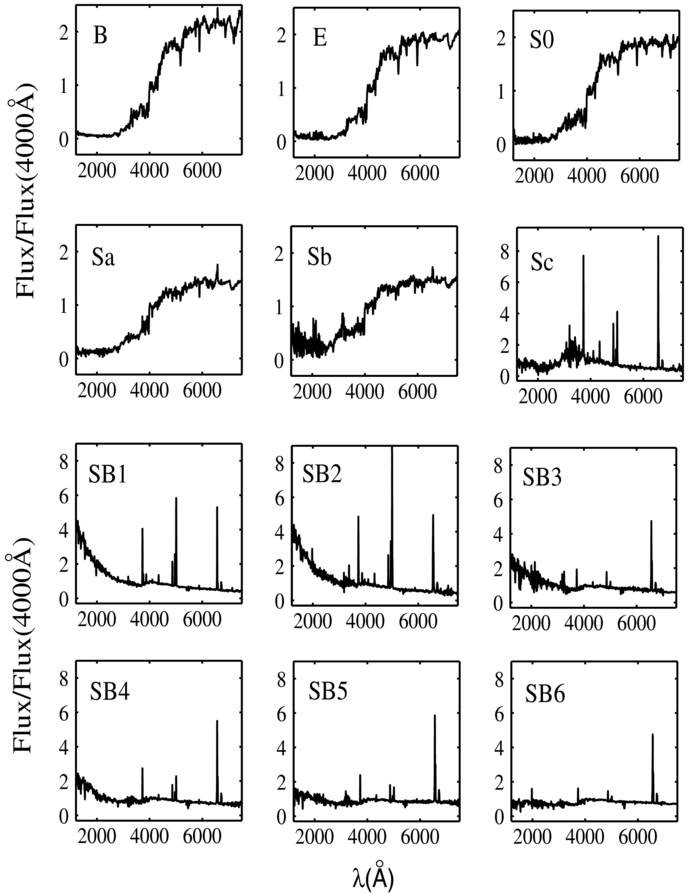
\includegraphics[width=0.5\textwidth]{images/k96.jpg}
        \caption{\citetalias{Kinney96} spectral templates for 12 types of galaxies from Fig. 1 of \citetalias{Hossein12}. The type of each template is shown in each frame. Plots B, E, S0, Sa, Sb and SC show spectra that belong to the quiescent types. Star-forming galaxy spectra are indicated with SB 1 to 6. Higher numbers represent more intrinsic extinction.}
        \label{fig: k96}
    \end{figure}
      
    \citetalias{Kinney96} used ultraviolet-optical spectra of 70 star-forming and quiescent nearby galaxies to produce a set of templates that contained 12 types of SEDs.
    These templates have been widely used in many studies to determine morphological types of galaxies or properties of specific types of galaxies~\citep[e.g.][]{Shakouri16, Paiano16, Laporte16, Holden16}.
    \citetalias{Kinney96} stated that these templates can also be used to classify the SEDs of high-redshift galaxies. 
    
    The 12 templates are divided based on their morphological types for quiescent galaxies or their extinction for starburst galaxies (Fig.~\ref{fig: k96}). 
    The quiescent group of galaxies includes Bulge (B), Elliptical (E), S0, Sa, Sb, and Sc galaxies.
    The bulge group represents galaxies similar to M31 and M81, whose UV and optical spectra are dominated by their bulge stellar populations.
    The starburst galaxies are divided into six groups (SB1 to SB6) based on their intrinsic extinctions ($E(B-V)$). 
    As Fig.~\ref{fig: k96} shows, SB1 galaxies have lower internal extinctions ($E(B-V) \simeq 0.05$), while SB6 galaxies have the highest amount of extinction ($E(B-V) \simeq 0.65$) among starburst galaxies. 
    In the quiescent (B to Sb) templates, the spectrum is redder; strong absorption lines and the 4000~\AA~break are distinguishable.
    The SEDs of starburst galaxies are flatter in the optical and near-infrared region than those of the quiescent types and show strong emission lines.
    For more details on each spectral type, we encourage readers to see \citetalias{Kinney96} and references therein. 
   The \citetalias{Kinney96} spectra span from $\sim1200$~\AA~to $10000$~\AA~with a resolution of $\sim 10$~\AA.
    However, in this work we only use $\sim1200< \lambda < 8000$~\AA~to train our networks; 
    this wavelength range was chosen due to availability of flux information in those wavelengths for all 12 templates. 

 \subsection{SED and Properties of the sample galaxies} 
    \citetalias{Hossein12} selected 142 galaxies from the spectroscopic campaign of the ESO GOODS-South field~\citep{Vanzella05, Vanzella06, Vanzella08}.
    The 142 galaxies were selected based on the availability of photometry from HST/ACS, VLT/ISAAC, and {\it Spitzer}/MIPS and IRAC (10--13 filters with $\sim 0.4<\lambda<24~\mu$m in the observed frame).
   Data from these instruments was necessary in order to have a complete picture of stellar population and star formation rate. 
    For each galaxy, a robust spectroscopic redshift and photometric measurements from the GOODS-MUSIC catalogue \citep{Santini09} was available.
   \citetalias{Hossein12} matched the resolution of the photometric data with \citetalias{Kinney96} data and used the photometry as inputs to the Code Investigating GALaxy Emission ({\em CIGALE});~\citep[][hereafter N09]{Noll09} to generate the best-fit SED for each galaxy. %PB20160623: I don't understand what "matched the point spread function of the photometric data with \citetalias{Kinney96} data" means.
   \citetalias{Hossein12} assumed decreasing SFR and visual attenuation ($\tau$) model, Salpeter initial mass function~\citep{Salpeter55}, and old stellar population with age of $\sim 10$~Gyr.% to find the best-fit SED for each galaxy. %%%Sr220616: moved the last sentence from the next paragraph to here.
   

    The fitting performed by \citetalias{Hossein12} produced the best SED match for each galaxy, with wavelength interval of 910~\AA~to $\sim 80$~cm\footnote{This wavelength interval is the default output of the {\em CIGALE} code}.
    \citetalias{Hossein12} derived physical properties of the galaxies such as SFR, age and stellar mass from these fitted SEDs. %%%Sr220616: change the previues sentence to matched to the new corrections.
    Some of these properties are shown in Tab.~\ref{tab: props}.
    In Sec.~\ref{sec: 1D}, we study these properties for each category.
    More details on creating SEDs and extracting information about galaxy properties using {\em CIGALE} can be found in \citetalias{Noll09} and \citetalias{Hossein12}.
    
       
    \begin{table}
\caption{Properties of \citetalias{Hossein12} galaxies from {\em CIGALE} output }   
\label{tab: props}
\centering
\begin{tabular}{l l l}
\hline\hline
\noalign{\smallskip}
Par. & Unit & Description\\
\noalign{\smallskip}
\hline
\noalign{\smallskip}
$t_{\,\mathrm{oSP}}$ & Gyr & age of old stellar population \\
$t_{\,\mathrm{ySP}}$ & Gyr & age of young stellar population \\
$f_\mathrm{burst}$ & --- & mass fraction of \\
& & young single population  \\
\noalign{\smallskip}
$t_{\,\mathrm{D4000}}$ & Gyr & D4000-related age \\
\noalign{\smallskip}
$M_\mathrm{star}$ & M$_\odot$ & total stellar mass  \\
SFR & M$_\odot$/yr & instantaneous SFR  \\
$A_\mathrm{FUV}$ & mag & attenuation at 1500\,\AA{} \\
\noalign{\smallskip}
\hline
\end{tabular}
\end{table}
    
    %%%Sr220616: Same as the intro section we did not test any thing here.
    We classify SEDs that were produced by \citetalias{Hossein12} using the created networks.
    %For testing the created networks, we use SEDs that were produced by \citetalias{Hossein12}. 
    These SEDs are publicly available~\footnote{All the \citetalias{Hossein12} produced SEDs can be found in \href{http://telbib.eso.org/detail.php?bibcode=2012AJ....144..172T}{ESO webpage}} in the form of flux per rest frame wavelength over a wide range of wavelengths.
    %Since we have used the \citetalias{Hossein12} SEDs to test the trained network, we only used the part of the SEDs that have the same wavelength range as the \citetalias{Kinney96} templates.  
    Since we have chosen the \citetalias{Hossein12} SEDs to be classified by the trained network, we only used the part of the SEDs that have the same wavelength range as the \citetalias{Kinney96} templates. 
